\documentclass[14pt,aspectratio=1610]{beamer}

\usepackage[brazil]{babel}
\usepackage[utf8]{inputenc}
%\UseRawInputEncoding
\usepackage[T1]{fontenc}
\usepackage{Sweave}
\usepackage{animate}
\usepackage{amsbsy}
\usepackage{amsfonts}
\usepackage{amsmath}
\usepackage{amssymb}
\usepackage{amsthm}
\usepackage[toc,page,title,titletoc]{appendix}
\usepackage[fixlanguage]{babelbib}
%\usepackage[pdftex]{color}
\usepackage{dsfont}
\usepackage{esvect}
\usepackage[labelfont=bf]{caption}
\usepackage{float}
\usepackage[Glenn]{fncychap}%Sonny %Conny %Lenny %Glenn %Renje %Bjarne %Bjornstrup
%\usepackage{geometry, calc, color, setspace}%
%\geometry{a4paper, headsep=1.0cm, footskip=1cm, lmargin=3cm, rmargin=2cm, tmargin=3cm, bmargin=2cm}
\usepackage{graphicx}
\usepackage{indentfirst}%Para indentar os parágrafos automáticamente
\usepackage{lipsum}
\usepackage{longtable}
\usepackage{mathtools}
\usepackage{listings}%Inserir codigo do R no latex
\usepackage{multirow}
\usepackage{multicol}
\usepackage{natbib}
\bibliographystyle{abbrvnat3}
\usepackage[figuresright]{rotating}
\usepackage{spalign}
%\usepackage{pgfpages}
\usepackage{pgfplots}
\usepackage{tikz}
\usepackage{color, colortbl}
\usepackage{ragged2e}%para justificar o texto dentro de algum ambiente
\definecolor{Gray}{gray}{0.9}
\definecolor{LightCyan}{rgb}{0.88,1,1}


\usepackage[all]{xy}
\usepackage{hyperref,bookmark}
\hypersetup{
  colorlinks=true,
  linkcolor=blue,
  citecolor=red,
  filecolor=blue,
  urlcolor=blue,
}

\usetheme{Madrid}
\usecolortheme[RGB={193,0,0}]{structure}

%\setbeamertemplate{footline}[frame number]
%\setbeamertemplate{footline}[text line]{%
%  \parbox{\linewidth}{\vspace*{-8pt}\hfill\date{}\hfill\insertshortauthor\hfill\insertpagenumber}}
\beamertemplatenavigationsymbolsempty
\renewcommand{\vec}[1]{\mbox{\boldmath$#1$}}
\newtheorem{Teorema}{Teorema}
\newtheorem{Proposicao}{Proposição}
\newtheorem{Definicao}{Definição}
\newtheorem{Corolario}{Corolário}
\newtheorem{Demonstracao}{Demonstração}
\newcommand{\bx}{\ensuremath{\bar{x}}}
\newcommand{\Ho}{\ensuremath{H_{0}}}
\newcommand{\Hi}{\ensuremath{H_{1}}}


\apptocmd{\frame}{}{\justifying}{} % Allow optional arguments after frame.

\title{MAF 261 - Estatística Experimental}
\author{Prof. Fernando de Souza Bastos}
\institute{Instituto de Ciências Exatas e Tecnológicas\texorpdfstring{\\ Universidade Federal de Viçosa}{}\texorpdfstring{\\ Campus UFV - Florestal}{}}
\date[\today]{}
\newcommand\mytext{Aulas 5, 6 e 7}
\newcommand\mytextt{Fernando de Souza Bastos}
\makeatletter
\setbeamertemplate{footline}
{
  \leavevmode%
  \hbox{%
  \begin{beamercolorbox}[wd=.333333\paperwidth,ht=2.25ex,dp=1ex,center]{author in head/foot}%
    \usebeamerfont{author in head/foot}\mytext
  \end{beamercolorbox}%
  \begin{beamercolorbox}[wd=.333333\paperwidth,ht=2.25ex,dp=1ex,center]{title in head/foot}%
    \usebeamerfont{title in head/foot}\mytextt
  \end{beamercolorbox}%
  % \begin{beamercolorbox}[wd=.333333\paperwidth,ht=2.25ex,dp=1ex,right]{date in head/foot}%
  %   \usebeamerfont{date in head/foot}\insertshortdate{}\hspace*{2em}
  %   \insertframenumber{} / \inserttotalframenumber\hspace*{2ex} 
  % \end{beamercolorbox}
  }%
  \vskip0pt%
}
\makeatother


\providecommand{\arcsin}{} \renewcommand{\arcsin}{\hspace{2pt}\textrm{arcsen}}
\providecommand{\sin}{} \renewcommand{\sin}{\hspace{2pt}\textrm{sen}}
%\newtheorem{Teorema}{Teorema}
%\newtheorem{Proposicao}{Proposição}
%\newtheorem{Definicao}{Definição}
%\newtheorem{Corolario}{Corolário}
%\newtheorem{Demonstracao}{Demonstração}

% Layout da pagina
\hypersetup{pdfpagelayout=SinglePage}
\begin{document}
\Sconcordance{concordance:Aula5_6e7.tex:Aula5_6e7.Rnw:%
1 248 1 1 19 1 4 49 1 1 4 6 0 1 9 7 0 1 1 3 0 1 2 10 1 1 9 1 2 660 1}


\frame{\titlepage}

\begin{frame}{}
\frametitle{\bf Sumário}
\tableofcontents
\end{frame}
\section{Teste de hipóteses para uma média populacional}
\subsection{Teste-z}
\begin{frame}{}
\frametitle{Testes para a Média de uma Distribuição Normal, Variância Conhecida}
\begin{block}{}
\justifying
Consideraremos teste de hipóteses acerca da média $\mu$ de uma única população normal, em que a variância da população $\sigma^{2}$ é conhecida. Consideraremos uma amostra aleatória $X_{1}, X_{2},\cdots, X_{n}$ sendo retirada da população. Lembre-se, a média amostral $\bar{X}$ é um estimador não tendencioso de $\mu$ com 
variância $\dfrac{\sigma^{2}}{n}.$
\end{block}
\end{frame}

\begin{frame}{}
\frametitle{}
\begin{block}{}
\justifying
Testamos as hipóteses $\Ho:\mu=\mu_{0}$ versus $\Hi$ que pode ser unilateral ou bilateral. A estatística do teste z para uma média é:
$$z_{cal}=\dfrac{\bx-\mu}{\dfrac{\sigma}{\sqrt{n}}}$$
Podemos encontrar o valor tabelado de z usando uma tabela apropriada a partir do nível de significância e da hipótese alternativa ou 
encontrar o valor - p e concluir de acordo com os resultados obtidos. Ao usar o valor tabelado, a regra de decisão será:
\begin{itemize}
\item $|z_{cal}|\geq z_{tab}\Rightarrow$ rejeitamos $\Ho;$
\item caso contrário não rejeitamos $\Ho.$
\end{itemize}
\end{block}
\end{frame}

\begin{frame}{}
\frametitle{Exemplo}
\begin{block}{}
\justifying
Os sistemas de escape da tripulação de uma aeronave funcionam por causa de um propelente sólido. A taxa de queima desse propelente é uma característica importante 
do produto. As especificações requerem que a taxa média de queima tem de ser $50$ centímetros por segundo. Sabemos que o desvio-padrão da taxa de queima é 
$\sigma = 2$ centímetros por segundo. O experimentalista decide especificar uma probabilidade do erro tipo I ou nível de significância de $\alpha = 0,05.$ Ele seleciona 
uma amostra aleatória de $n = 25$ e obtém uma taxa média amostral de queima de $\bx = 51,3$ centímetros por segundo. Que conclusões poderiam ser tiradas?
\end{block}
\end{frame}

\begin{frame}{}
\frametitle{Exemplo}
\begin{block}{}
\justifying
\begin{align*}
H_{0}: \mu&=50 cm/s\\ 
H_{1}: \mu&\neq 50 cm/s
\end{align*}
A estatística do teste z para uma média é:
$$z_{cal}=\dfrac{51.3-50}{\dfrac{2}{\sqrt{25}}}=3.25$$
O p-valor do teste é p-valor$=2*(1-\Phi(3.25))=0.0012.$ Os limites das regiões critícas são $z_{tab}=z_{0.025}=1.96$ e $-z_{tab}=-z_{0.025}=-1.96$
\end{block}
\end{frame}

\begin{frame}{}
\frametitle{Exemplo}
\begin{block}{}
\justifying
\begin{figure}
\centering
\begin{tikzpicture}[xscale=1.5, yscale=7, declare function={stdnorm(\x) = 1/(sqrt(2*pi))*exp(-0.5*(pow(\x,2)));}]
\fill[gray] (-2.5,0) -- plot [domain=-2.5:-3/2, samples=50] (\x, {stdnorm(\x)}) -- (-3/2,0) -- cycle;
\fill[gray] (3/2,0) -- plot [domain=3/2:5/2, samples=50] (\x, {stdnorm(\x)}) -- (5/2,0) -- cycle;
\draw [thick, domain=-2.5:2.5, samples=50] plot (\x, {stdnorm(\x)});
\draw [->] (-3,0) -- (3,0) ;
\node [below right] at (3,0) {$z$} ;
\draw [dashed] (0,0) -- (0,{stdnorm(0)}) ;
\draw [dashed] (-3/2,0) -- (-3/2,{stdnorm(-3/2)}) ;
\draw [dashed] (3/2,0) -- (3/2,{stdnorm(3/2)}) ;
\node [below] at (0,0) {$0$};
\node [below] at (-3/2,0) {$-1.96$};
\node [below] at (3/2,0) {$1.96$};
\node [above] at (-2.5,0.1) {\small{RR$\Ho$}};
\node [above] at (2.5,0.1) {\small{RR$\Ho$}};
\node [above] at (-1,0.5) {\small{RNR$\Ho$}};
\node [above] at (2,0.5) {$z_{cal}=3.25$};
\node [above] at (2,0.4) {p-valor$=0.0012$};
\node [above] at (2,0.3) {$\alpha=0.05$};
%\draw[->] (-2.7,0.15) .. controls (.-2,.2) .. (-1.9, 0.03);
\draw[->] (-2.2,0.15) to [out=20,in=90] (-1.9,0.02);
\draw[->] (2.2,0.15) to [out=160,in=90] (1.9,0.02);
\draw[->] (-0.6,0.55) to [out=0,in=90] (0.1,0.3);
%\draw [->,thick] (2.7,0.15) to [out=120,in=0] (2.3,0.3)
%to [out=0,in=90] (1.9,0.03);
%\draw (0,0) .. controls (0,4) and (4,0) .. (4,4)
%\draw[->] ( 3,0.15) .. controls (. 30,.2) .. (1.9, 0.03);
%\node at (1.8,{stdnorm(2.3)}) {\small{$\alpha/2$}};
%\node at (-1.8,{stdnorm(2.3)}){\small{$\alpha/2$}};
\end{tikzpicture}
%\caption{Região crítica para $\Ho: \mu = 50$ versus $\Hi: \mu \neq 50$ e $n = 25$}
\end{figure}
\end{block}
\vspace{-0.5cm}
\pause
\begin{block}{}
\textbf{Conclusão:} Como o p-valor é menor que $\alpha$ rejeita-se $\Ho$ ao nível de $\alpha=5\%$ de significância. De outra forma, como $|z_{cal}|>|z_{tab}|$ rejeita-se 
$\Ho$ ao nível de $\alpha=5\%$ de significância.
\end{block}
\end{frame}

\subsection{Teste-t}
\begin{frame}{}
\frametitle{Testes para a Média de uma Distribuição Normal, Variância desconhecida}
\begin{block}{}
\justifying
A aplicação do teste t é indicada quando o tamanho amostral é igual ou inferior a 30 elementos. Para amostras com tamanho superior a 30, recomenda-se o teste Z. 
\end{block}
\pause
\begin{block}{}
\justifying
Ressalta-se que o uso do teste t pressupõe distribuição normal com variância populacional desconhecida. 
\end{block}
\end{frame}

\begin{frame}{}
\frametitle{Teste de hipóteses para uma média populacional}
\begin{block}{}
\justifying
Este teste é usado para verificar se a média de uma característica de uma população assume um valor especificado, 
digamos $\mu_{0}$. Para aplicação deste teste devemos selecionar uma amostra aleatória de tamanho $n$ da população. 
Digamos que os elementos amostrais sejam; $X_{1},X_{2},\cdots,X_{n}.$ Com base nestes elementos amostrais, 
calculamos a sua média, $\bx$, e seu desvio padrão, $s$. Estas estatísticas são então utilizadas para calcular o valor de $t_{cal}$ 
usando a expressão:
$$t_{cal}=\dfrac{\bx-\mu}{\dfrac{s}{\sqrt{n}}}$$
Esta estatística t, tem distribuição t de Student com $n-1$ graus de liberdade. 
\end{block}
\end{frame}

\begin{frame}[fragile]{}
\frametitle{Teste de hipóteses para uma média populacional}
\begin{center}
\setkeys{Gin}{width=0.5\linewidth}
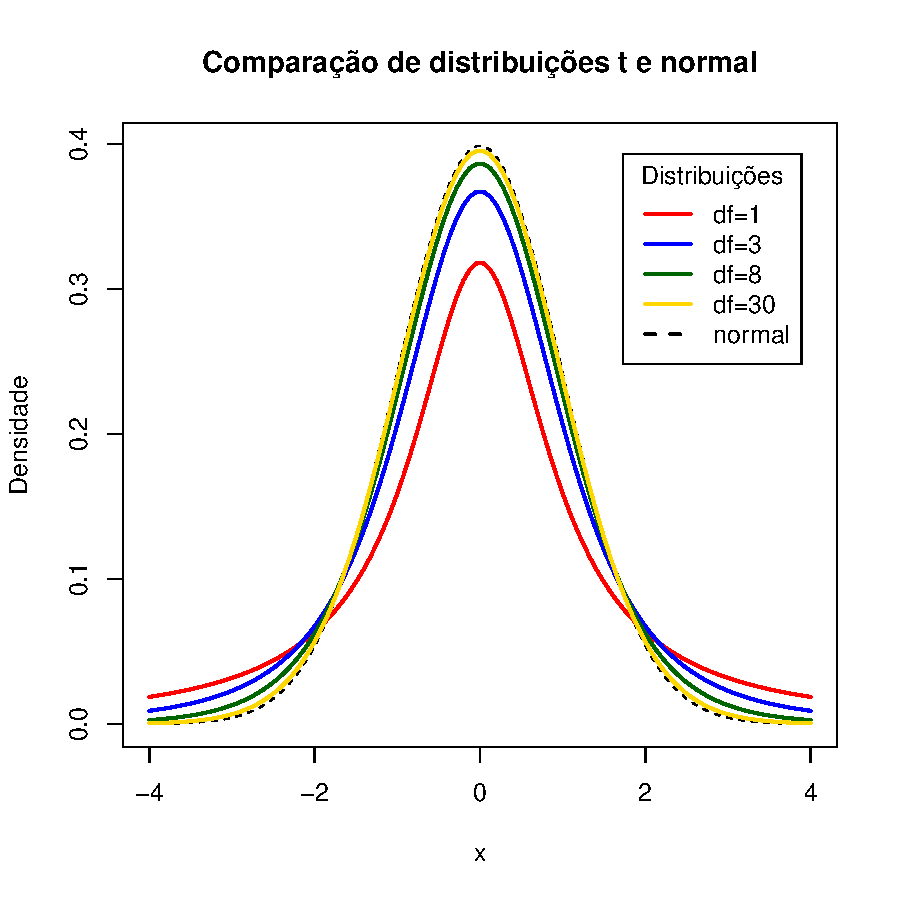
\includegraphics{Aula5_6e7-001}
\end{center}
\end{frame}

\begin{frame}{}
\frametitle{}
\begin{block}{}
\justifying
Para decidirmos entre Rejeitar ou Não-Rejeitar $\Ho$, comparamos o valor de t com o valor tabelado de t obtido por 
$t_{tab}=t_{\alpha}(n-1).$ Depois de obtido o valor calculado e o valor tabelado de t, usamos a seguinte regra
decisória:
\begin{itemize}
\item $|t_{cal}|\geq t_{tab}\Rightarrow$ rejeitamos $\Ho;$
\item caso contrário não rejeitamos $\Ho.$
\end{itemize}
\end{block}
\end{frame}

\begin{frame}{}
\frametitle{Exemplo}
\begin{block}{}
\justifying
A disponibilidade crescente de materiais leves com alta resistência tem revolucionado o projeto e a fabricação de tacos de golfe, particularmente os direcionadores. 
Tacos com cabeças ocas e faces muito finas podem resultar em tacadas muito mais longas, especialmente para jogadores de habilidades modestas. Isso é causado 
parcialmente pelo ``efeito mola'' que a face fina impõe à bola. Bater na bola de golfe com a cabeça do taco e medir a razão entre a velocidade de saída da bola e a 
velocidade de chegada pode quantificar esse efeito mola. A razão de velocidades é chamada de coeficiente de restituição do taco. 
\end{block}
\end{frame}

\begin{frame}{}
\frametitle{Exemplo}
\begin{block}{}
\justifying
Um experimento foi feito, em que $15$ tacos direcionadores, produzidos por determinado fabricante de tacos, foram selecionados ao acaso e seus coeficientes de 
restituição foram medidos. No experimento, bolas de golfe foram atiradas a partir de um canhão de ar, de modo que a velocidade de chegada e a taxa de giro da bola 
poderiam ser precisamente controladas. É de interesse determinar se há evidência (com $\alpha = 0,05$) que suporte a afirmação de que o coeficiente médio de restituição 
excede $0,82.$ As observações seguem:
\begin{table}[]
\begin{tabular}{ccccc}
0,8411 &0,8191 &0,8182 &0,8125 &0,8750 \\
0,8580 &0,8532 &0,8483 &0,8276 &0,7983 \\
0,8042 &0,8730 &0,8282 &0,8359 &0,8660 
\end{tabular}
\end{table}
A média e o desvio-padrão da amostra são $\bx = 0,83725$ e $s = 0,02456.$
\end{block}
\end{frame}

\begin{frame}[fragile]{}
\frametitle{Exemplo}
\begin{block}{}
\begin{Schunk}
\begin{Sinput}
> dados <- c(0.8411,0.8191,0.8182,0.8125,0.8750,0.8580,
+            0.8532,0.8483,0.8276,0.7983,0.8042,0.8730,
+            0.8282,0.8359,0.8660)
\end{Sinput}
\end{Schunk}
\begin{Schunk}
\begin{Sinput}
> # Gráfico de probabilidade (QQ)
> qqnorm(dados, 
+        main = "", xlab = "Quantis teóricos N(0,1)", 
+        pch = 20,
+        ylab = "coeficiente médio de restituição",
+        xlim=c(-2,2),
+        ylim=c(0.75,0.9))
> qqline(dados, lty = 2, col = "red")
\end{Sinput}
\end{Schunk}
\end{block}
\end{frame}

\begin{frame}[fragile]{}
\frametitle{Exemplo}
\begin{block}{}
O gráfico de probabilidade normal dos dados suporta a suposição de que o coeficiente médio de restituição é normalmente distribuído.
\end{block}
\vspace{-1.2cm}
\begin{center}
\setkeys{Gin}{width=0.5\linewidth}
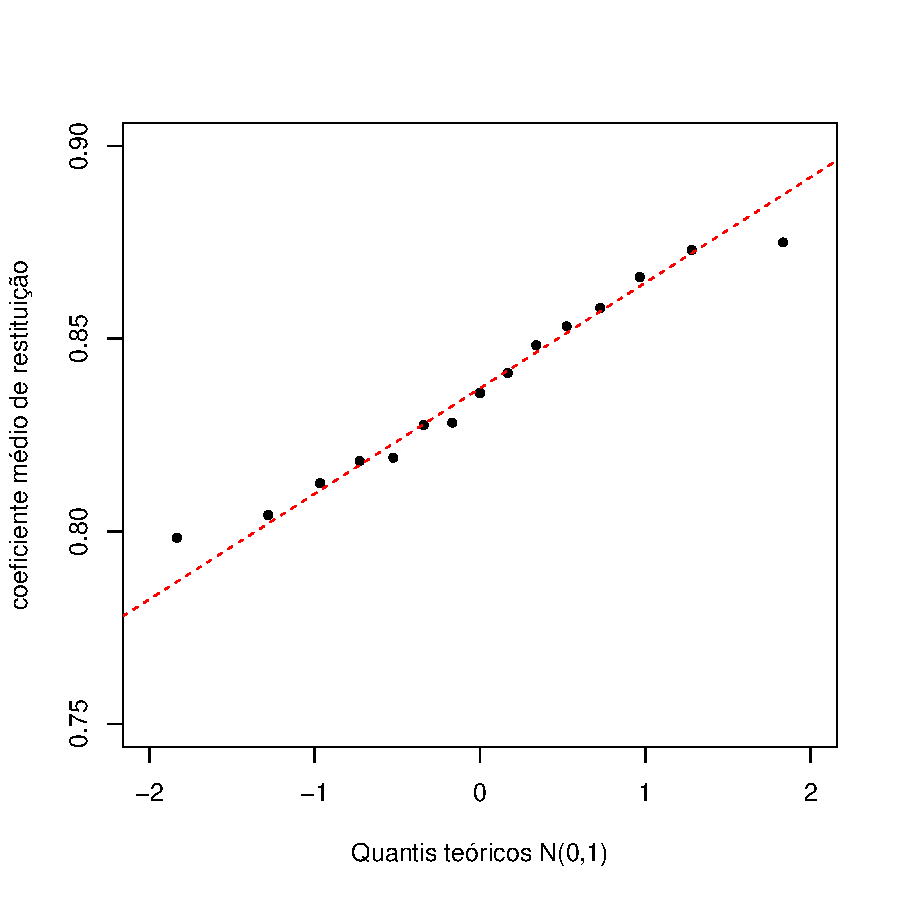
\includegraphics{Aula5_6e7-plot}
\end{center}
\end{frame}


% \begin{frame}{}
% \frametitle{Exemplo}
% \begin{block}{}
% \justifying
% O gráfico de probabilidade normal dos dados suporta a suposição de que o coeficiente médio de restituição é normalmente distribuído.
% \begin{figure}[H]
%     \centering
%     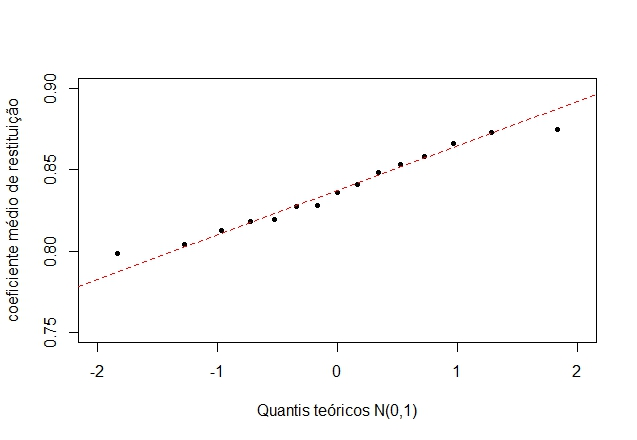
\includegraphics[scale=0.5]{Prob_Normal1}
%     %\caption{Legenda}
%     %\label{figRotulo}
%   \end{figure}
% \end{block}
% \end{frame}

\begin{frame}{}
\frametitle{Exemplo}
\begin{block}{}
\justifying
Logo, podemos utilizar o teste t:
\begin{align*}
H_{0}: \mu&=0.82 \\ 
H_{1}: \mu&> 0.82
\end{align*}
A estatística do teste t para uma média é:
$$t_{cal}=\dfrac{0.83725-0.82}{\dfrac{0.02456}{\sqrt{15}}}=2.72$$
O limite da região critíca é $t_{tab}=t_{0.05}(14)=1,76$

\textbf{Conclusão:} Como $|t_{cal}|>|t_{tab}|$ rejeita-se $\Ho$ ao nível de $\alpha=5\%$ de significância.
\end{block}
\end{frame}

\section{Teste de hipóteses para duas médias populacionais}
\begin{frame}{}
\frametitle{Teste de hipóteses para duas médias populacionais}
\begin{block}{}
\justifying
O objetivo deste teste é verificar se duas populações, digamos população 1 e população 2 apresentam um mesmo valor médio para uma determinada característica, isto é, deseja-se verificar se $\mu_{1}=\mu_{2}$. Com esta finalidade é necessário obter uma amostra de cada população. Estas duas amostras podem ser relacionadas ou não, ou seja, podem ser dependentes ou 
independentes uma da outra. Esta distinção no relacionamento das duas amostras gera 
dois testes distintos. Além disso, podemos ter variâncias populacionais conhecidas, iguais ou diferentes, ou variâncias populacionais desconhecidas, que também podem ser iguais ou 
diferentes. Para cada caso também temos um teste. Antes de ver tais testes, precisamos conhecer o teste F de Snedecor.
\end{block}
\end{frame}

\subsection{Teste F para Comparação de Variâncias de Duas Populações}
\begin{frame}{}
\frametitle{Teste F para Comparação de Variâncias de Duas Populações}
\begin{block}{}
\justifying
Este teste é indicado para verificar se duas populações, digamos 1 e 2, apresentam igual valor para o parâmetro variância. Em termos de hipóteses estatísticas teríamos:

\begin{flalign}
\begin{aligned} 
	\begin{cases}
H_{0}: \sigma_{1}^{2}=\sigma_{2}^{2}\\
H_{1}:\sigma_{1}^{2}>\sigma_{2}^{2}
\end{cases}
\end{aligned}
\quad\textrm{ou}\quad
\begin{aligned}
\begin{cases}
H_{0}: \sigma_{1}^{2}=\sigma_{2}^{2}\\
H_{1}:\sigma_{1}^{2}<\sigma_{2}^{2}
\end{cases} \\
\end{aligned}
\quad\textrm{ou}\quad
\begin{aligned}
\begin{cases}
H_{0}: \sigma_{1}^{2}=\sigma_{2}^{2}\\
H_{1}:\sigma_{1}^{2}\neq\sigma_{2}^{2}
\end{cases} \\
\end{aligned}
\end{flalign}
\end{block}
\end{frame}

\begin{frame}{}
\frametitle{}
\begin{block}{}
\justifying
A estatística F usada para decidir entre Rejeitar ou Não-Rejeitar $\Ho$ é dada pelo quociente entre as duas estimativas de variância, ou seja:
$$F_{cal}=\dfrac{S_{1}^{2}}{S_{2}^{2}}$$
Sob a hipótese de nulidade, este quociente tem distribuição F, de Fisher-Snedecor, com $n_{1}$ e $n_{2}$ graus de liberdade, ou seja a distribuição de probabilidades 
da estatística $F$ depende dos números de graus de liberdade $n_{1}$ e $n_{2}$. A conclusão do teste é feita mediante a comparação do valor de $F_{cal}$ com o 
valor de $F_{tab}=F_{\alpha}(n_{1},n_{2}).$ Se $F_{cal}>F_{tab}$ Rejeita-se $\Ho$ ao nível $\alpha$ de probabilidade. Caso contrário Não-Rejeita-se $\Ho.$
\end{block}
\end{frame}

\begin{frame}{}
\frametitle{Exemplo}
\begin{block}{}
\justifying
Com o intuito de controlar a homogeneidade da produção de certas partes ao longo do tempo, amostras semanais são retiradas da produção corrente. Uma primeira 
amostra, de dez elementos, forneceu média $\bx=284.55$ e desvio padrão $s_{1}=0.320$, ao passo que, numa segunda amostra, forneceu, nas mesmas unidades, os seguintes valores:
\begin{table}[]
\begin{tabular}{ccccccc}
             284.6 & 283.9 & 284.8 & 285.2 & 284.3 & 283.7 & 284.0\\ 
\end{tabular}
\end{table}
Ao nível de $5\%$ de significância, podemos concluir que a semana 2 apresentou maior variabilidade que a semana 1?
\end{block}
\end{frame}

\begin{frame}{}
\frametitle{Exemplo}
\begin{block}{}
\justifying
\begin{align*}
H_{0}: \sigma_{1}^{2}&=\sigma_{2}^{2} \\ 
H_{1}: \sigma{1}^{2}&<\sigma_{2}^{2}
\end{align*}
\begin{align}
F_{cal}=\dfrac{S_{1}^{2}}{S_{2}^{2}}=\dfrac{0,289}{0,1024}=2,82
\end{align}
O limite da região critíca é $F_{tab}=F_{6,9}(0,05)=3,37$\\
\textbf{Conclusão:} Como $F_{cal}<F_{tab}$ não rejeita-se $\Ho$ ao nível de $\alpha=5\%$ de significância. 
\end{block}
\end{frame}

\subsection{Variâncias populacionais conhecidas}
\begin{frame}{Variâncias populacionais conhecidas}
\frametitle{}
\begin{block}{}
\justifying
Suponha $P_{1}\sim N(\mu_{1},\sigma_{1}^{2})$ e $P_{2}\sim N(\mu_{2},\sigma_{2}^{2}).$ Queremos testar a hipótese $H_{0}:\mu_{1}=\mu_{2}.$ Se as variâncias populacionais são conhecidas (iguais ou diferentes), a estatística $$Z_{cal}=\dfrac{\bar{X}-\bar{Y}}{\sqrt{\dfrac{\sigma_{1}^{2}}{n}+\dfrac{\sigma_{2}^{2}}{m}}}$$ tem distribuição normal padrão, sob a hipótese nula $H_{0},$ e poderia ser usada para testar $\Ho$ contra $\Hi$.
\end{block}
\end{frame}

\begin{frame}{}
\frametitle{}
\begin{block}{}
\justifying
Contudo, nas situações de interesse prático, as variâncias não são conhecidas, devendo ser substituídas por estimativas convenientes. Aqui, a distribuição $t$ de Student desempenha papel importante. Vejamos os próximos slides!
\end{block}
\end{frame}

\subsection{Variâncias Desconhecidas e Desiguais}
\begin{frame}{Variâncias Desconhecidas e Desiguais}
\frametitle{}
\begin{block}{}
\justifying
Quando a hipótese de igualdade de variâncias for rejeitada pelo teste F, devemos usar a estatística $$t_{cal}=\dfrac{\bar{X}-\bar{Y}}{\sqrt{\dfrac{S_{1}^{2}}{n}+\dfrac{S_{2}^{2}}{m}}}$$ o número de graus de liberdade é dado aproximadamente por:
\vspace{-0.2cm}
$$df=\dfrac{(A+B)^{2}}{\dfrac{A^{2}}{n-1}+\dfrac{B^{2}}{m-1}},\ 
A=\dfrac{S_{1}^{2}}{n},\ B=\dfrac{S_{2}^{2}}{m}$$
\end{block}\pause
\vspace{-0.5cm}
\begin{block}{}
Como esse valor é geralmente fracionário, arredonde para o inteiro mais próximo
para obter o número de graus de liberdade.
\end{block}
\end{frame}

\subsection{Variâncias Desconhecidas, porém iguais}
\begin{frame}{}
\frametitle{Teste de hipóteses para o caso de duas amostras independentes}
\begin{block}{}
\justifying
Duas amostras são ditas serem independentes quando não existe nada que as relacione. Nesta situação, os valores amostrais foram obtidos em conjuntos amostrais distintos, ou seja, os elementos amostrais que originaram os valores de uma amostra são distintos dos elementos amostrais que originaram a segunda amostra.
\end{block}
\end{frame}

\begin{frame}{}
\frametitle{}
\begin{block}{}
\justifying
Conforme mencionado anteriormente, para comparar as médias das duas populações, toma-se uma amostra de cada população. Suponha que as amostras geradas sejam $X_{11},X_{12},\cdots,X_{1n}$ e $X_{21},X_{22},\cdots,X_{2m}$, onde o tamanho das amostras podem ser diferentes, ou seja, n pode ser diferente de m. Para cada amostra, então calcula-se a sua média e variância. Se as variâncias populacionais são iguais (faça um teste f para verificar isso), um estimador comum para a variância é obtido tomando-se uma média ponderada das estimativas de variância obtidas para as duas amostras. O tamanho da amostra é utilizado como um peso para o cálculo desta variância média ponderada.
\end{block}
\end{frame}

\begin{frame}{}
\frametitle{}
\begin{block}{}
\justifying
A obtenção de um estimador comum para a variância pressupõe que a variância das duas populações sejam idênticas, ou seja $\sigma^{2}_{1}=\sigma^{2}_{2}.$ A fórmula do estimador comum é:
$$s_{c}^{2}=\dfrac{(n_{1}-1)s_{1}^{2}+(n_{2}-1)s_{2}^{2}}{n_{1}+n_{2}-2}$$ em que $s_{1}^{2}$ e $s_{2}^{2}$ são as variâncias amostrais das populações 1 e 2, respectivamente. 
\end{block}
\end{frame}

\begin{frame}{}
\frametitle{}
\begin{block}{}
\justifying
Uma vez obtidas estas estimativas, calcula-se o valor da estatística 
t dada por:
$$t_{cal}=\dfrac{(\bx_{1}-\bx_{2})-(\mu_{1}-\mu_{2})}{\sqrt{s_{c}^{2}\Biggl(\frac{1}{n_{1}}+\frac{1}{n_{2}}\Biggl)}}$$ 
Esta estatística tem distribuição t de Student com $(n_{1}+n_{2}-2)$ graus de liberdade. Faz-se então a comparação do valor 
calculado de t com o valor tabelado dado por $t_{tab}=t_{\alpha}(n_{1}+n_{2}-2),$ usando a regra:
\begin{itemize}
\item $|t_{cal}|\geq t_{tab}\Rightarrow$ rejeitamos $\Ho;$
\item caso contrário não rejeitamos $\Ho.$
\end{itemize}
\end{block}
\end{frame}

\begin{frame}{}
\frametitle{Exemplo}
\begin{block}{}
\justifying
Os dados que seguem referem-se a cinco determinações da resistência de dois tipos de concreto. Ao nível de $5\%$ de significância, há evidência de que o concreto 
1 seja mais resistente que o concreto 2?
\begin{table}[]
\begin{tabular}{c|ccccc}
Concreto 1 & 54 & 55 & 58 & 51 & 57 \\ \hline
Concreto 2 & 50 & 54 & 56 & 52 & 53
\end{tabular}
\end{table}
\end{block}
\end{frame}

\begin{frame}{}
\frametitle{Exemplo}
\begin{block}{}
{\bf *}Procedemos o teste F e não rejeitamos $\Ho:\sigma_{1}^{2}=\sigma_{2}^{2}$
\justifying
\begin{align*}
H_{0}: \mu_{1}&=\mu_{2} \\ 
H_{1}: \mu_{1}&> \mu_{2}
\end{align*}
$$t_{cal}=\dfrac{(\bx_{1}-\bx_{2})-(\mu_{1}-\mu_{2})}{\sqrt{s_{c}^{2}\Biggl(\frac{1}{n_{1}}+\frac{1}{n_{2}}\Biggl)}}=
                 \dfrac{(55-53)}{\sqrt{6.25\Biggl(\frac{1}{5}+\frac{1}{5}\Biggl)}}=1.265$$
O limite da região critíca é $t_{tab}=t_{0.05}(8)=1,86$\\
\textbf{Conclusão:} Como $|t_{cal}|<|t_{tab}|$ não rejeita-se $\Ho$ ao nível de $\alpha=5\%$ de significância.
\end{block}
\end{frame}

\section{Teste de hipóteses para o caso de duas amostras dependentes}
\begin{frame}{}
\frametitle{Teste de hipóteses para o caso de duas amostras dependentes}
\begin{block}{}
\justifying
Duas amostras de elementos são ditas serem dependentes quando existe algo que as relacione. Por exemplo, se os valores de duas amostras foram obtidos de um mesmo conjunto de elementos amostrais, podemos dizer que as duas amostras de valores são dependentes uma vez que foram tomados de um conjunto de elementos
amostrais comum.
\end{block}
\pause
\begin{block}{}
\justifying
O objetivo neste caso é verificar se houve alteração na média de uma população
quando a mesma é avaliada sob duas condições diferentes. Cada condição representa
uma população distinta, embora se suponha que os elementos populacionais sejam os
mesmos nas duas condições.
\end{block}
\end{frame}

\begin{frame}{}
\frametitle{}
\begin{block}{}
\justifying
Para verificar se houve alteração na média, avalia-se uma característica de interesse do pesquisador num conjunto de elementos amostrais tomados ao acaso na população quando a mesma esteja sob a condição 1. Digamos que a avaliação da característica resulte nos seguintes valores amostrais $X_{11},X_{12},\cdots,X_{1n}$.
\end{block}
\end{frame}

\begin{frame}{}
\frametitle{}
\begin{block}{}
\justifying
Depois de feita esta avaliação, os elementos amostrais que originaram a primeira amostra, sejam submetidos à condição 2. Os mesmos elementos amostrais são novamente avaliados para a mesma característica na nova condição 2. Digamos que esta nova avaliação resulte nos seguintes valores amostrais $X_{21},X_{22},\cdots,X_{2n}$. 
Se a condição 2 não tiver nenhum efeito, espera-se que em média os valores observados nas duas condições sejam iguais.
\end{block}
\end{frame}

\begin{frame}{}
\frametitle{}
\begin{block}{}
\justifying
Em termos de desvios, se a alteração das condições não resultasse em nenhum
efeito significativo, poderíamos dizer que a diferença entre os valores observados na
primeira condição e na segunda condição seria em média igual a zero. Portanto para
verificar se houve alteração na média de uma população avaliada em duas condições
diferentes, pode-se testar a hipótese de que o desvio médio ser estatisticamente igual a
zero.
\end{block}
\end{frame}

\begin{frame}{}
\frametitle{}
\begin{block}{}
\justifying
Portanto, a partir de duas amostras obtém-se uma outra baseada nos desvios, conforme é mostrado a seguir.
\begin{table}[]
\begin{tabular}{ccccc}
\hline \hline
Elemento amostral $i$& 1              &   2            & $\cdots$  & $n$ \\
\hline
amostra 1                    & $X_{11}$ & $X_{12}$ & $\cdots$ & $X_{1n}$ \\
amostra 2                    & $X_{21}$ & $X_{22}$ & $\cdots$ & $X_{2n}$ \\
\hline
 $d_{i}=X_{1i}-X_{2i}$& $d_{1}$   & $d_{2}$    & $\cdots$ & $d_{n}$\\
\hline
\end{tabular}
\end{table}
Apresentado desta forma, o teste t para duas amostras dependentes reduz-se teste t para uma média populacional, visto anteriormente. No presente caso, deseja-se testar
se a média dos desvios é igual por exemplo a um valor $\mu_{0}$.
\end{block}
\end{frame}

\begin{frame}{}
\frametitle{}
\begin{block}{}
\justifying
Para decidir entre Rejeitar ou Não-Rejeitar a hipótese de nulidade, deve-se calcular o valor da estatística t dada por
\begin{align*}
t_{cal}=\dfrac{\bx-\mu}{\dfrac{s}{\sqrt{n}}}\quad \textrm{em que}\quad \bx=\dfrac{\displaystyle \sum_{i=1}^{n}d_{i}}{n}\quad \textrm{e}\quad 
s^{2}=\dfrac{\displaystyle \sum_{i=1}^{n}d_{i}^{2}-\dfrac{(\displaystyle \sum_{i=1}^{n}d_{i})^{2}}{n}}{n-1}
\end{align*}
Sob $\Ho$, esta estatística t tem distribuição t de Student com $n-1$ graus de liberdade. A comparação deste valor calculado com o valor de $t_{tab}$ dado por 
$t_{tab}=t_{\alpha}(n-1)$ nos leva a conclusão do teste.
\end{block}
\end{frame}

\begin{frame}{}
\frametitle{Exemplo}
\begin{block}{}
\justifying
Com o objetivo de avaliar se determinado produto químico é eficiente para repelir insetos domésticos, foi realizada uma 
contagem do número de insetos, antes e após a aplicação deste produto químico, em 7 residências. O número de insetos 
observado em cada residência foi
\begin{table}[]
\begin{tabular}{c|ccccccc}
             Residência & 1 & 2 & 3 & 4 & 5 & 6 & 7\\ \hline
Antes da aplicação & 8 & 6 & 7 & 8 & 9 & 6 & 7 \\ 
Após a aplicação    & 4 & 0 & 3 & 5 & 3 & 4 & 2 \\ \hline
Diferença ($d_{i}$)      & 4 & 6 & 4 & 3 & 6 & 2 & 5 \\ \hline
\end{tabular}
\end{table}
Por meio destes dados e ao nível de $5\%$ de probabilidade, é possível concluir, em termos médios, que o produto 
utilizado é eficiente para repelir insetos?
\end{block}
\end{frame}

\begin{frame}{}
\frametitle{Exemplo}
\begin{block}{}
\justifying
\begin{align*}
H_{0}: \mu_{d}&=0 \\ 
H_{1}: \mu_{d}&> 0
\end{align*}
$$t_{cal}=\dfrac{(4.286-0)}{\sqrt{\dfrac{2.24}{7}}}=7.58$$
O limite da região critíca é $t_{tab}=t_{0.05}(6)=1,94$\\
\textbf{Conclusão:} Como $|t_{cal}|>|t_{tab}|$ rejeita-se $\Ho$ ao nível de $\alpha=5\%$ de significância.
\end{block}
\end{frame}

\section{Teste \texorpdfstring{$\chi^{2}$}{$x^{2}$} para a variância}
\begin{frame}{}
\frametitle{Teste $\chi^{2}$ para a variância}
\begin{block}{}
\justifying
Suponha que desejamos testar a hipótese de que a variância de uma população normal $\sigma^{2}$ seja igual a um valor específico, como $\sigma^{2}_{0}$, ou 
equivalentemente, que o desvio-padrão $\sigma$ seja igual a $\sigma_{0}.$ Seja $X_{1},X_{2},\cdots,X_{n}$ uma amostra aleatória de $n$ observações, proveniente 
dessa população. Para testar 
\begin{align*}
H_{0}: \sigma^{2}=\sigma_{0}^{2}\\
H_{1}:\sigma^{2}>\sigma_{0}^{2}
\end{align*}
usaremos a estatística de teste:
\begin{align}\label{qui}
\chi^{2}_{cal}=\dfrac{(n-1)S^{2}}{\sigma_{0}^{2}}
\end{align}
%Se a hipótese nula $H0: \sigma^{2}=\sigma_{0}^{2}$ for verdadeira, então a estatística de teste $\chi^{2}$ , definida na Equação (\ref{qui}), segue a distribuição qui-quadrado, 
%com $n - 1$ graus de liberdade.
\end{block}
\end{frame}
\begin{frame}{}
\frametitle{Teste $\chi^{2}$ para a variância}
\begin{block}{}
\justifying
Se a hipótese nula $H_{0}: \sigma^{2}=\sigma_{0}^{2}$ for verdadeira, então a estatística de teste $\chi^{2}$ , definida na Equação (\ref{qui}), segue a distribuição qui-quadrado, 
com $n - 1$ graus de liberdade.
\end{block}
\end{frame}

\begin{frame}{}
\frametitle{Exemplo}
\begin{block}{}
\justifying
Uma máquina de enchimento automático é usada para encher garrafas com detergente líquido. Uma amostra aleatória de 20 garrafas resulta em uma variância amostral de volume de enchimento de $ s^{2}= 0,0153 ml^{2}$. Se a variância do volume de enchimento exceder 0,01, existirá uma proporção inaceitável de garrafas cujo enchimento não foi completo e cujo enchimento foi em demasia. Há evidência nos dados da amostra sugerindo que o fabricante tenha um problema com garrafas cheias com falta e excesso de detergente? Use $\alpha = 0,05$ e considere que o volume de enchimento tenha uma distribuição normal.
\end{block}
\end{frame}

\begin{frame}{}
\frametitle{Exemplo}
\begin{block}{}
\justifying
\begin{align*}
H_{0}: \sigma^{2}&=0.01 \\ 
H_{1}: \sigma^{2}&>0.01
\end{align*}
\begin{align}
\chi^{2}_{cal}=\dfrac{(n-1)S^{2}}{\sigma_{0}^{2}}=\dfrac{19\times0.0153}{0.01}=29.07
\end{align}
O limite da região critíca é $\chi_{tab}=\chi_{0.05}(19)=30,14$\\
\textbf{Conclusão:} Como $|\chi_{cal}|<|\chi_{tab}|$ não rejeita-se $\Ho$ ao nível de $\alpha=5\%$ de significância. Logo, não há forte evidência de um problema com 
garrafas preenchidas incorretamente.
\end{block}
\end{frame}

\section{Testes para a Proporção de uma População}
\begin{frame}{Distribuição de Bernoulli}
\frametitle{}
\begin{block}{}
\justifying
Muitos experimentos são tais que os resultados apresentam ou não uma determinada
característica. Por exemplo:
\begin{enumerate}
\item uma moeda é lançada: o resultado ou é cara, ou não (ocorrendo, então, coroa);\pause
\item um dado é lançado: ou ocorre face 5 ou não (ocorrendo, então, uma das faces
1, 2, 3, 4 ou 6);\pause
\item uma peça é escolhida ao acaso de um lote contendo 500 peças: essa peça é
defeituosa ou não;\pause
\item uma pessoa escolhida ao acaso dentre 1.000 é ou não do sexo masculino;\pause
\item uma pessoa é escolhida ao acaso entre os moradores de uma cidade e verifica-se
se ela é favorável ou não a um projeto municipal.
\end{enumerate}
\end{block}
\end{frame}

\begin{frame}{Distribuição de Bernoulli}
\frametitle{}
\begin{block}{}
\justifying
Em todos esses casos, estamos interessados na ocorrência de sucesso (cara, face 5
etc.) ou fracasso (coroa, face diferente de 5 etc.). Para cada experimento acima, podemos definir uma v.a. $X,$ que assume apenas dois valores: 1, se ocorrer sucesso, e 0, se ocorrer fracasso. Indicaremos por $p$ a probabilidade de sucesso, isto é, 
$P(sucesso)=P(S) = p,\ 0<p<1.$
\end{block}
\end{frame}

\begin{frame}{}
\frametitle{}
\begin{block}{}
\justifying
{\bf Definição:} Uma variável aleatória $X,$ que assume apenas os valores $0$ e $1,$ com função de probabilidade $(x, p(x))$ tal que
\begin{align*}
p(0)&=P(X=0)=1-p;\\
p(1)&=P(X=1)=p
\end{align*}
é chamada variável aleatória de Bernoulli. Note que,
\begin{align*}
E(X)&=p;\\
V(X)&=p(1-p)
\end{align*}
\end{block}
\pause
\begin{block}{}
{\bf Observação:} Experimentos que resultam numa v.a. de Bernoulli são chamados ensaios
de Bernoulli. Usamos a notação $X\sim Ber(p)$ para indicar uma v.a. com distribuição de Bernoulli com parâmetro p. 
\end{block}
\end{frame}

\begin{frame}{Distribuição Binomial}
\frametitle{}
\begin{block}{}
\justifying
Imagine, agora, que repetimos um ensaio de Bernoulli $n$ vezes, ou, de maneira
alternativa, obtemos uma amostra de tamanho $n$ de uma distribuição de Bernoulli.
Suponha ainda que as repetições sejam independentes, isto é, o resultado de um ensaio
não tem influência nenhuma no resultado de qualquer outro ensaio. Uma amostra
particular será constituída de uma seqüência de sucessos e fracassos, ou, alternativamente, de uns e zeros.
\end{block}
\end{frame}

\begin{frame}{}
\frametitle{Distribuição Binomial}
\begin{block}{}
\justifying
Imagine, agora, que repetimos um ensaio de Bernoulli $n$ vezes, ou, de maneira
alternativa, obtemos uma amostra de tamanho $n$ de uma distribuição de Bernoulli.
Suponha ainda que as repetições sejam independentes, isto é, o resultado de um ensaio
não tem influência nenhuma no resultado de qualquer outro ensaio. Uma amostra
particular será constituída de uma seqüência de sucessos e fracassos, ou, alternativamente, de uns e zeros.
\end{block}
\end{frame}

\begin{frame}{}
\frametitle{Distribuição Binomial}
\begin{block}{}
\justifying
Por exemplo, repetindo um ensaio de Bernoulli cinco vezes $(n = 5),$ um particular resultado pode ser FSSFS ou a quíntupla ordenada $(0, 1, 1, 0, 1).$ Usando a notação 
$P(S) = p,$ a probabilidade de tal amostra será:
$$(1-p)pp(1-p)p=p^{3}*(1-p^{2})$$
O número de sucessos nessa amostra é igual a 3, sendo 2 o número de fracassos.
\end{block}
\end{frame}

\begin{frame}{}
\frametitle{Distribuição Binomial}
\begin{block}{}
\justifying
Designamos por $X$ o número total de sucessos em $n$ ensaios de Bernoulli, com
probabilidade de sucesso $p, 0 < p < 1.$ Os possíveis valores de $X$ são $0, 1, 2, ..., n$ e os pares $(x, p(x)),$ onde $p(x) = P(X = x),$ constituem a chamada distribuição binomial.
\end{block}
\end{frame}

\begin{frame}{}
\frametitle{Distribuição Binomial}
\begin{block}{}
\justifying
Assim, numa seqüência de n ensaios de Bernoulli, a probabilidade de obter $x$ sucessos (e portanto $n-x$ fracassos), $x = 0,1,2, ..., n,$ com $P(S) = p, P(F) = 1-p = q,$ é dado por $p^{x}(1-p)^{n-x}=p^{x}q^{n-x},$ devido à independência dos ensaios. Mas qualquer seqüência com $x$ sucessos e $n-x$ fracassos terá a mesma probabilidade. Portanto resta saber quantas seqüências com a propriedade especificada podemos formar. É fácil ver que existem $$\binom{n}{x}=\dfrac{n!}{x!(n-x)!},$$ logo, 
$$P(X=x)=\binom{n}{x}p^{x}q^{n-x},\ x = 0,1,2, ..., n.$$
\end{block}
\end{frame}

\begin{frame}{}
\frametitle{Distribuição Binomial}
\begin{block}{}
\justifying
Se X tem distribuição binomial com parâmetros $n$ e $p,$ indicamos $X\sim Bin(n,p).$ Nesse caso, 
\begin{align*}
E(X)&=np;\\
V(X)&=np(1-p)
\end{align*}
\end{block}
\end{frame}

\begin{frame}{Testes para a Proporção de uma População}
\frametitle{}
\begin{block}{}
\justifying
Em muitos problemas de engenharia, estamos preocupados com uma variável aleatória que siga a distribuição binomial. Por exemplo, considere um processo de produção 
que fabrica itens que são classificados como aceitáveis ou defeituosos. É geralmente razoável modelar a ocorrência de defeitos com a distribuição binomial, em que o 
parâmetro binomial $p$ representa a proporção de itens defeituosos produzidos. Consequentemente, muitos problemas de decisão em engenharia incluem teste de 
hipóteses para $p.$
\end{block}
\end{frame}

\begin{frame}{}
\frametitle{}
\begin{block}{}
\justifying

Consideraremos o teste
\begin{align*}
H_{0}: p=p_{0}\\
H_{1}:p\neq p_{0}
\end{align*}
Seja $X$ o número de observações em uma amostra aleatória de tamanho $n$ que pertence 
à classe associada a $p.$ Então, se a hipótese nula $\Ho: p = p_{0}$ for verdadeira, teremos $X \sim N[np_{0}, np_{0}(1 - p_{0})],$ aproximadamente. Para testar 
$\Ho: p = p_{0},$ calcule a estatística de teste:
\begin{align}\label{proporcao}
z_{cal}=\dfrac{\bx-np_{0}}{\sqrt{np_{0}(1 - p_{0})}},\ \bx=n\hat{p}
\end{align}
Se a hipótese nula $H0:p=p_{0}$ for verdadeira, então a estatística de teste $z$ , definida na Equação (\ref{proporcao}), segue a distribuição normal padrão.
\end{block}
\end{frame}

\begin{frame}{}
\frametitle{Exemplo}
\begin{block}{}
\justifying
Um fabricante de semicondutores produz controladores usados em aplicações no motor de automóveis. O consumidor requer que a fração de\-fei\-tuo\-sa em uma etapa crítica de fabricação não exceda 0,05 e que o fabricante demonstre uma capacidade de processo nesse nível de qualidade, usando $\alpha = 0,05.$ O fabricante de 
semicondutores retira uma amostra aleatória de 200 aparelhos e encontra que quatro deles são defeituosos. O fabricante pode demonstrar uma capacidade de processo 
para o consumidor?
\end{block}
\end{frame}

\begin{frame}{}
\frametitle{Exemplo}
\begin{block}{}
\justifying
\begin{align*}
H_{0}: p&=0,05 \\ 
H_{1}: p&<0,05
\end{align*}
\begin{align}
z_{cal}=\dfrac{\bx-np_{0}}{\sqrt{np_{0}(1 - p_{0})}}=\dfrac{4-200\times(0,05)}{\sqrt{200\times0,05\times(0,95)}}=-1,95
\end{align}
O valor p é dado por valor-p$=\Phi(-1,95)=0,0256$\\
\textbf{Conclusão:} Como p-valor$<\alpha=0,05$ rejeita-se $\Ho$ ao nível de $\alpha=5\%$ de significância. Concluímos que a fração defeituosa do processo, $p,$ é 
menor do que 0,05 e, portanto, o processo é capaz.
\end{block}
\end{frame}

% \begin{frame}[fragile]{}
% \frametitle{}
% \begin{block}{}
% <<echo=TRUE, results=hide>>=
% #------------------------------------------------
% # dir.create("exemplos")
% # png(file="exemplos/qnorm%1d.png", width=500, 
% #height=250)
% # par(mar=c(4,4,1,1))
% #------------------------------------------------
% @ 
% \end{block}
% \end{frame}
% 
% \begin{frame}[fragile]{}
% \frametitle{}
% \begin{block}{}
% <<echo=TRUE, results=hide>>=
% #-----------------------------------------------
% for(q in seq(0, 4,l=100)){
%   curve(dnorm(x, 0, 1), -5, 5, ylab="f(z)", xlab="z")
%   x <- seq(0, q, by=0.01)
%   fx <- dnorm(x, 0, 1)
%   polygon(c(x, rev(x)),
%           c(fx, rep(0, length(fx))),
%           col="gray90")
%   abline(v=0, lty=2)
%   Pr <- round(pnorm(q, 0, 1)-0.5, digits=3)
%   qq <- round(q, digits=3)
%   legend("topleft", bty="n", fill="gray90",
%          legend=substitute(P(0<~Z<=~q)==Pr, 
%                            list(q=qq, Pr=Pr)))}
% dev.off()
% #-----------------------------------------------
% @ 
% \end{block}
% \end{frame}
% 
% \begin{frame}[fragile]{}
% \frametitle{}
% \begin{block}{}
% <<echo=TRUE, results=hide>>=
% #-----------------------------------------------
% require(xtable)
% options(OutDec=",")
% q <- seq(0,3.99,by=0.01)
% p <- pnorm(q)-0.5
% m <- matrix(p, byrow=TRUE, ncol=10)
% rownames(m) <- gsub("\\.", ",", 
%                     formatC(seq(0,3.9,0.1),
%                             dig=1, format="f"))
% colnames(m) <- 0:9/100
% #-----------------------------------------------
% @
% \end{block}
% \end{frame}
% 
% \begin{frame}[fragile]{}
% \frametitle{}
% \begin{block}{}
% \begin{center}
% \animategraphics[controls, loop, width=0.75\textwidth]{10}{exemplos/qnorm}{1}{100}
% \end{center}
% \end{block}
% \end{frame}
% 
% \begin{frame}[fragile]{}
% \frametitle{}
% \begin{block}{}
% \begin{center}
% \small\addtolength{\tabcolsep}{-3pt}
% {\footnotesize
% <<echo=false, results=tex>>=
% #-----------------------------------------------------------------------------
% print(xtable(m, digits=5), floating=FALSE)
% #-----------------------------------------------------------------------------
% @ 
% }
% \end{center}
% \end{block}
% \end{frame}



\end{document}
